\clearpage
\subsection*{PPL de Transport – Minimizare}
\paragraph{}
Chișinău și Bălți sunt centre de aprovizionare cu \textbf{produse alimentare} pentru centrele de desfacere
Ialoveni, Căușeni și Leova. 
Transportul se poate efectua de la oricare centru A\textsubscript{i} către oricare centru D\textsubscript{j}, existând un cost unitar C\textsubscript{ij}, al 
transportului unui bun de la centrul A\textsubscript{i} către centrul Dj. Astfel, costul total al 
transportului este proporţional cu cantitatea de bunuri transportate între sursă 
şi destinaţie. Datele problemei se află în Tabel ~\ref{tab:minimizare}. Unitățile ce țin de marfă sunt în camionae cu marfa respectivă.

\paragraph{}
\begin{table}[h]
\captionsetup{singlelinecheck = false, justification=raggedright}
\caption{Problema de minimizare a cheltuielilor pe transport}
\label{tab:minimizare} 
\begin{center}
\begin{tabular}{|l|l|l|l|l|}
\cline{2-4}
\multicolumn{1}{l|}{Ai\textbackslash{}Dj}&Ialoveni&Căușeni&Leova&\multicolumn{1}{l}{Disponibil}\\
\hline
Chișinău&\multicolumn{1}{l}{15}&\multicolumn{1}{l}{70}&100&100\\
\cline{1-1}\cline{5-5}
Bălți&\multicolumn{1}{l}{140}&\multicolumn{1}{l}{200}&200&200\\
\hline
\multicolumn{1}{l|}{Cererea}&150&75&75&\multicolumn{1}{l}{300}\\
\cline{2-4}
\end{tabular}
\end{center}
\end{table}


\paragraph{}
\begin{figure}[h]
\begin{center}
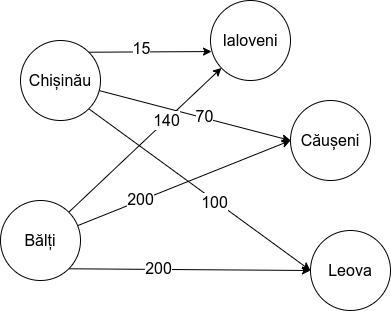
\includegraphics[width=12cm]{drumuri}
\caption{Reprezentarea grafica a costurilor de transport} 
\label{fig:drumuri}
\end{center}
\end{figure}

\paragraph{}
Dupa cum se vede din Figura ~\ref{fig:drumuri} și din tabelul
~\ref{tab:minimizare} problema data are 6 variaile și nu ar pute fi rezolvată
prin metoda grafică dacă nu am aduce-o mai întâi la 2 variablie.


\paragraph{}
\begin{table}[h]
\captionsetup{singlelinecheck = false, justification=raggedright}
\caption{Reducerea de la 6 variabile la 2}
\label{tab:reducere_min} 
\begin{center}
\begin{tabular}{|l|l|l|l|l|} 
\hline
Ai\textbackslash{}Dj& Ialoveni & Căușeni & Leova & Disponibil\\ 
\hline
\multirow{2}{*}{Chișinău} & 15 & 70& 100& \multirow{2}{*}{100}  \\
  & x  & y & 100 - x - y &  \\ 
\hline
\multirow{2}{*}{Bălți} & 140& 200  & 200& \multirow{2}{*}{200}  \\
  & 150 - x  & 75 - y  & x + y - 25  &  \\ 
\hline
Cererea & 150& 75& 75 & 300 \\
\hline
\end{tabular}
\end{center}
\end{table}


\paragraph{}
	Pentru a putea rezolva problema prin metoda grafică am notat prin x prima variabilă x\textsubscript{11} și y a doua variabilă x\textsubscript{12} astfel putem scrie funcția de calcul a prețului în felul următor:
\begin{equation*}
Z = 15x + 70y +10000 -100x -100y +21000 -140x + 15000 - 200y - 5000 + 200x + 200y
\end{equation*}

\paragraph{Modelul matematic}
Este necesar de gasit valorile nenegative ale variabilelor x și y pentru care funcția Z atinge valoarea minimă.

\begin{equation*}
Z = -25 x - 30 y + 41000 \rightarrow MIN
\end{equation*}

Restricții:

\begin{gather*}
	x + y \leq 100, \\
	x \leq 150, \\
	y \leq 75, \\
	x + y \geq 25, \\
	x \geq 0, \;
	y \geq 0.
\end{gather*}

\paragraph{}
Rezolvare. Construim poligonul convex al soluțiilor.

\begin{gather*}
	x + y = 100 \; (L1); \\
	x = 150 \; (L2); \\
	y = 75 \; (L3); \\
	x + y = 25 \; (L4); \\
	x = 0; \;
	y = 0.
\end{gather*}


\begin{figure}[h]
\begin{center}
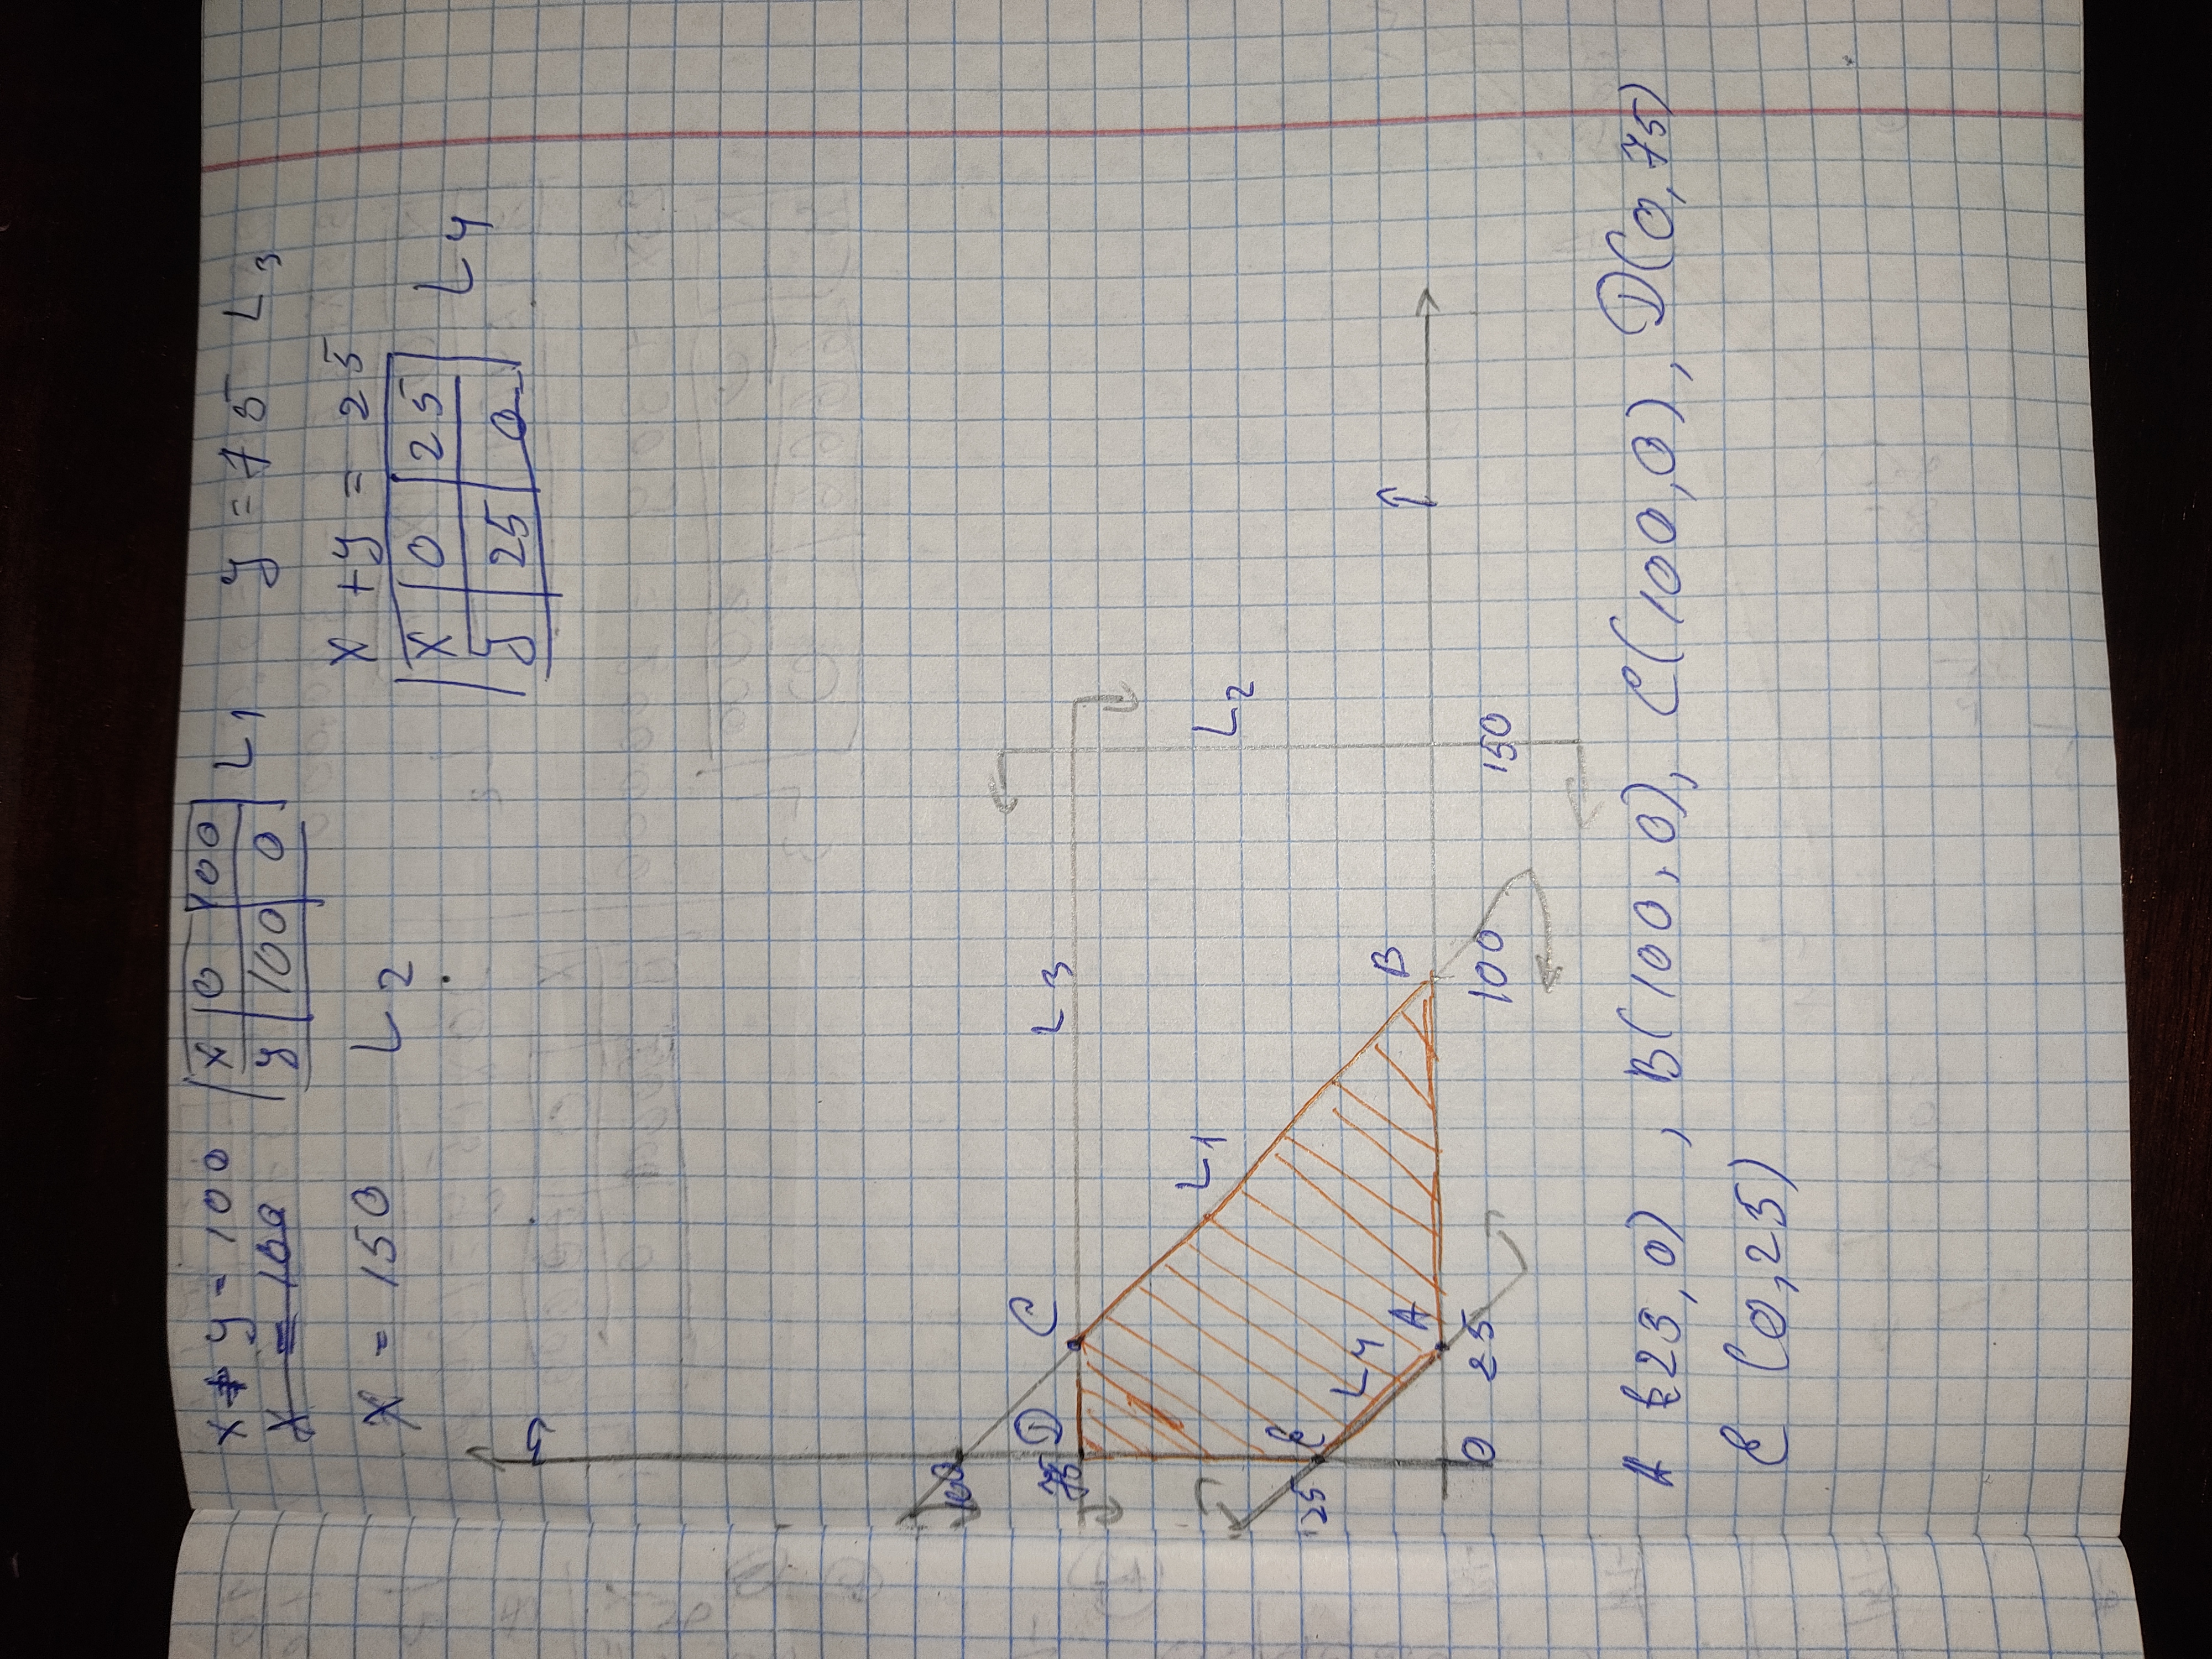
\includegraphics[width=15cm, angle=-90]{minimizare}
\caption{Poligonul convex solutiilor admisibile} 
\label{fig:minimizare}
\end{center}
\end{figure}

\paragraph{}

\paragraph{}
Poligonul convex are următoarele vârfuri: A(25,0), B(100,0), C(25,75), D(0,75), E(0,25)
\begin{gather*}
	Z(A) = -25 * 25 + -30 * 0 + 41000 = 40375 \\
	Z(B) = -25 * 100 + -30 * 0 + 41000 = 38500 \\
	Z(C) = -25 * 25 + -30 * 75 + 41000 = 38125 \\
	Z(D) = -25 * 0 + -30 * 75 + 41000 = 38750 \\
	Z(E) = -25 * 0 + -30 * 25 + 41000 = 40250 \\
\end{gather*}
După cum se observă vârful C este soluția optimă a problemei.

\paragraph{}
Rezultatul pentru problema de 2 variabile este x = 25; y = 75. Introducând valorile x și y în funcția liniară, obținem
\begin{equation*}
	Z\textsubscript{MIN} = -25 * 25 - 30 * 75 + 41000 = 38125 \\\end{equation*}
Acum putem substitui valorile x și y în tabelul inițial pentru a obține rezultatul final, valorile celor 6 variabile.

\paragraph{}
\begin{table}[h]
\captionsetup{singlelinecheck = false, justification=raggedright}
\caption{Introducea variabilelor x și y în tabel}
\label{tab:variabile_min} 
\begin{center}
\begin{tabular}{|l|l|l|l|l|} 
\hline
Ai\textbackslash{}Dj& Ialoveni & Căușeni & Leova & Disponibil\\ 
\hline
\multirow{4}{*}{Chișinău} & 15 & 70& 100 & 100 \\ 
\cline{2-5}
& x& y & 100 - x - y & \multirow{3}{*}{5625} \\
& 25 & 75& 0& \\
& 375 & 5250& 0& \\ 
\hline
\multirow{4}{*}{Bălți}& 140& 200 & 200 & 200 \\ 
\cline{2-5}
& 150 - x& 75 - y& x + y - 25& \multirow{3}{*}{32500}\\
& 125& 0& 75 & \\
& 17500& 0 & 15000 & \\ 
\hline
Cererea & 150& 75& 75& 300 \\
\hline
\end{tabular}
\end{center}
\end{table}

\paragraph{Răspuns }
În tabelul ~\ref{tab:variabile_min} am restabilit cele 6 variabile: 25, 75, 0, 125, 0, 75. Și le putem introduce în funcția Z:
\begin{gather*}
	Z= 
	c\textsubscript{11} * x\textsubscript{11} +  
	c\textsubscript{12} * x\textsubscript{12} +  
	c\textsubscript{13} * x\textsubscript{13} +  
	c\textsubscript{21} * x\textsubscript{21} +  
	c\textsubscript{22} * x\textsubscript{22} +  
	c\textsubscript{33} * x\textsubscript{33}  \rightarrow MIN  \\
Z\textsubscript{MIN} = 375 + 5250 + 0 + 17500 + 0 + 15000 = \\
= 5625 + 32500 = 38125
\end{gather*}
